\chapter{Reliability}
\section{Esercizio 1}
Calcolare \textbf{Reliability} e \textbf{MTTF} per il sistema il cui Reilability Block Diagram è rappresentato nell'immagine sottostante. Assumere che tutti i componenti sono identici e falliscono randomicamente con tasso di fallimento \textit{$\lambda$}.
\begin{figure}[H]
	\centering
	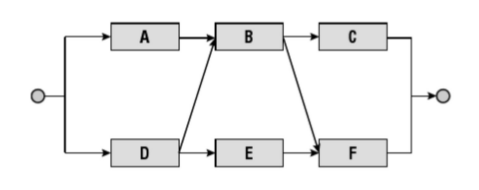
\includegraphics[width=1\textwidth]{img/hw5/es1.png}
	\caption{\textit{Reliability Block Diagram Es.1}}
\end{figure}
\subsection{Svolgimento}
Dalla traccia si evince che la \textit{reliability} di un singolo blocco del sistema in questione ha andamento esponenziale ed è:
\begin{equation*}
	R_i = e^{-\lambda*t}
\end{equation*}
\subsubsection{Success Diagram}
Non è ancora possibile riconoscere una serie da un parallelo in questo caso, quindi una prima cosa da fare è ricavare un \textit{success diagram}, ovvero un sistema composto da un parallelo di serie. Le serie sono anche dette \textit{success path} e coincidono con tutti i percorsi possibili dall'ingresso all'uscita del sistema. 
\begin{figure}[H]
	\centering
	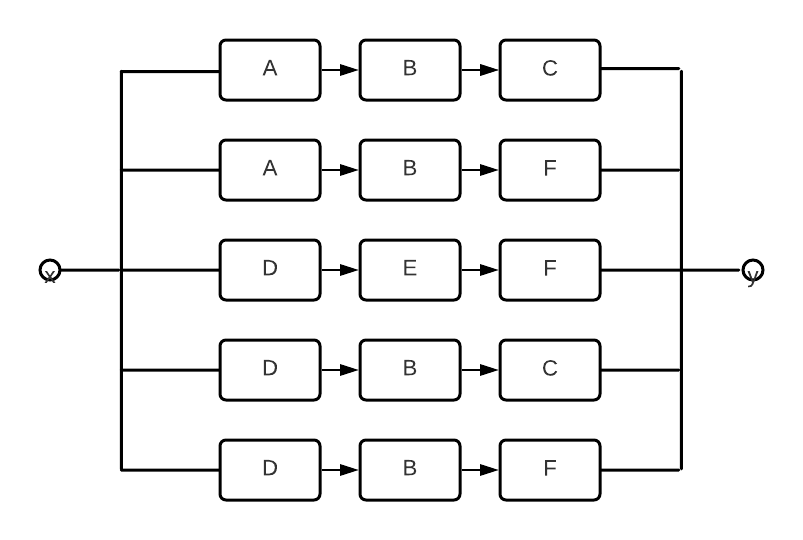
\includegraphics[width=0.7\textwidth]{img/hw5/success_diag.png}
	\caption{\textit{Success Diagram Es.1}}
\end{figure}
\begin{equation*}
	Rsys \leq 1 - \prod_{i=1}^{N}(1 - Rpath_i)
\end{equation*}
Con $N$ pari al numero di serie del diagramma, e $Rpath_i$ la reliability del path i-esimo.
\\Nel caso specifico dell'esercizio:
\begin{equation*}
	Rsys \leq 1 - [(1 - R_A*R_B*R_C)*(1-R_A*R_B*R_F)*(1-R_D*R_E*R_F)*(1-R_D*R_B*R_C)*(1-R_D*R_B*R_F)]
\end{equation*}
In questo modo è possibile ricavare agevolmente una reliability che sarà un upper bound per quella effettiva del sistema. Difatti i vari path non sono tra di loro indipendenti, dato che il fallimento di un blocco potrebbe interessare più di una serie.
\begin{equation*}
	Rsys \leq 1 - (1 - e^{-3\lambda*t})^{5}
\end{equation*}
\subsubsection{Conditioning}
La tecnica del \textbf{conditioning} consente di ricavare la reliability di un sistema facendo uso della formula del teorema di Bayes:
\begin{equation*}
	P(A) = \sum_{i = 1}^{N}P(A/B_i)P(B_i)
\end{equation*}
In poche parole, dato il sistema, viene supposto che uno dei suoi componenti $R_m$ (quello più critico per l'analisi) sia fallito o meno. Otteniamo quindi due versioni del diagramma iniziale:
\begin{enumerate}
	\item \textit{con componente selezionato up (circuito chiuso)}.
	\item \textit{con componente selezionato down (circuito aperto)}.
\end{enumerate}
\begin{equation*}
	Rsys = Rsys_1 + Rsys_2 = R_m*P(sys\,works|m\,up) + (1 - R_m)*P(sys\,works|m\,down)
\end{equation*}
\subsubsection{Conditioning sul blocco E}
\begin{figure}[H]
	\centering
	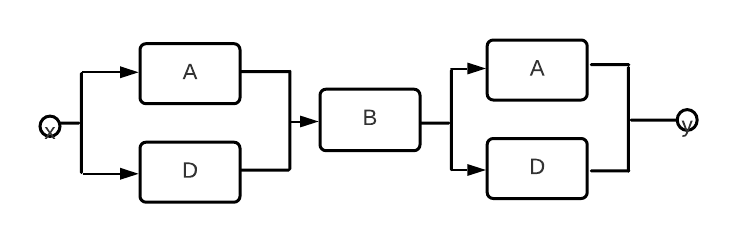
\includegraphics[width=0.7\textwidth]{img/hw5/e_down.png}
	\caption{\textit{Diagramma con Blocco E down Es.1}}
\end{figure}
Il sistema è composto da 2 paralleli in serie con il blocco B. La reliability totale può essere calcolata agevolmente sfruttando le formule di blocchi in serie e in parallelo.

\begin{equation*}
	Rsys_2 = (1-R_E)*P(sys\,works|E\,down)
\end{equation*}
\begin{equation*}
	\begin{split}
		Rsys_2 &= (1-R_E)*\{[1-(1-R_A)*(1-R_D)]*R_B*[1-(1-R_C)*(1-R_F)]\} \\
		&= (1-e^{-\lambda t})*[1-(1-e^{-\lambda t})^{2}]^{2}*e^{-\lambda t} \\
		&= (1-e^{-\lambda t})*[1-(1+e^{-2\lambda t}-2e^{-\lambda t})]^{2}*e^{-\lambda t} \\
		&= (1-e^{-\lambda t})*[-e^{-2\lambda t}+2e^{-\lambda t}]^{2}*e^{-\lambda t} \\
		&= (1-e^{-\lambda t})*[e^{-4\lambda t}+4e^{-2\lambda t}-4e^{-3\lambda t}]*e^{-\lambda t} \\
		&=(1-e^{-\lambda t})*[e^{-5\lambda t}+4e^{-3\lambda t}-4e^{-4\lambda t}] \\
		&= [e^{-5\lambda t}+4e^{-3\lambda t}-4e^{-4\lambda t}] - [e^{-6\lambda t}+4e^{-4\lambda t}-4e^{-5\lambda t}] \\
		&= 4e^{-3\lambda t}-8e^{-4\lambda t}+5e^{-5\lambda t}-e^{-6\lambda t}
	\end{split}
\end{equation*}
\begin{figure}[H]
	\centering
	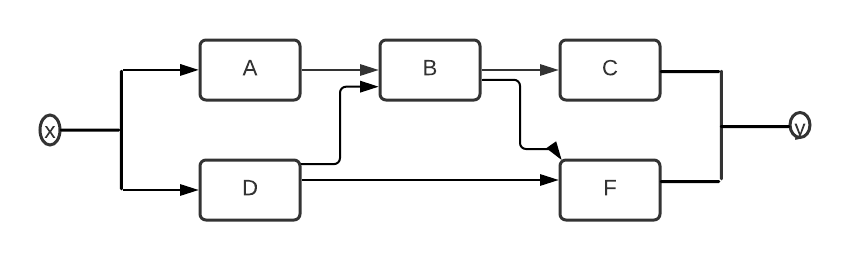
\includegraphics[width=0.7\textwidth]{img/hw5/e_up.png}
	\caption{\textit{Diagramma con Blocco E up Es.1}}
\end{figure}
\begin{equation*}
	Rsys_1 = R_E*P(sys\,works|E\,up)
\end{equation*}
Tuttavia il sistema così ottenuto deve ancora essere condizionato, visto che non essendo combinazione di serie e/o paralleli non è possibile ricavare immediatamente la probabilità condizionata.
\subsubsection{Conditioning sul blocco B - E up}
\begin{figure}[H]
	\centering
	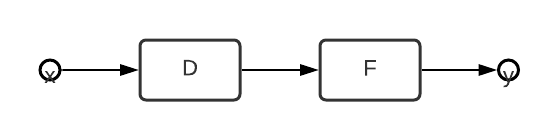
\includegraphics[width=0.7\textwidth]{img/hw5/b_down.png}
	\caption{\textit{Blocco E up e Blocco B down Es.1}}
\end{figure}
\begin{figure}[H]
	\centering
	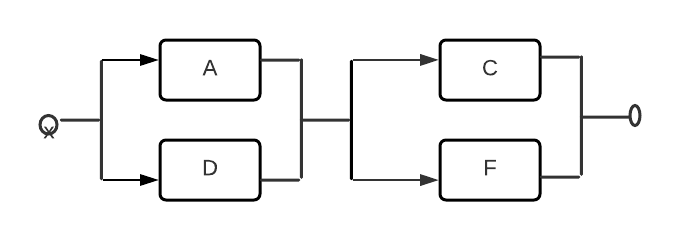
\includegraphics[width=0.7\textwidth]{img/hw5/b_up.png}
	\caption{\textit{Blocco E up e Blocco B up Es.1}}
\end{figure}
\begin{equation*}
	P(sys\,works|E\,up) = P(sys\,works|B\,down)*P(B\,down)+P(sys\,works|B\,up)*P(B\,up) =
\end{equation*}

\begin{equation*}
	\begin{split}
	P(sys\,works|E\,up) &= (1-R_B)*R_D*R_F + R_B*[1-(1-R_A)*(1-R_D)]*[1-(1-R_C)*(1-R_F)]  \\
	&= (1-e^{-\lambda t})*e^{-2\lambda t} + e^{-\lambda t}*[1-(1-e^{-\lambda t})^{2}]^{2} \\
	&= e^{-2\lambda t} - e^{-3\lambda t} + e^{-\lambda t}*[e^{-4\lambda t}+4e^{-2\lambda t}-4e^{-3\lambda t}] \\
	&= e^{-2\lambda t} - e^{-3\lambda t} + e^{-5\lambda t}+4e^{-3\lambda t}-4e^{-4\lambda t} \\
	&= e^{-2\lambda t} + 3e^{-3\lambda t} -4e^{-4\lambda t} +e^{-5\lambda t} 
	\end{split}
\end{equation*}
Dunque otteniamo che :
\begin{equation*}
	\begin{split}
		Rsys_1 &= e^{-\lambda t}*[e^{-2\lambda t} + 3e^{-3\lambda t} -4e^{-4\lambda t} +e^{-5\lambda t}] \\
		&=  e^{-3\lambda t} + 3e^{-4\lambda t} -4e^{-5\lambda t} +e^{-6\lambda t}
	\end{split}
\end{equation*}
Quindi la \textbf{reliability totale} del sistema sarà:
\begin{equation*}
	\begin{split}
		Rsys &= Rsys_1 + Rsys_2 \\
		&= 4e^{-3\lambda t}-8e^{-4\lambda t}+5e^{-5\lambda t}-e^{-6\lambda t} + e^{-3\lambda t} + 3e^{-4\lambda t} -4e^{-5\lambda t} +e^{-6\lambda t} \\
		&= 5e^{-3\lambda t}-5e^{-4\lambda t}+ e^{-5\lambda t}
	\end{split}
\end{equation*}
Mentre il \textbf{MTTF - Mean Time To Failure} è:
\begin{equation*}
	MTTF = \int_{0}^{\infty} Rsys(t)dt = \frac{5}{3\lambda}-\frac{5}{4\lambda}+\frac{1}{5\lambda}
\end{equation*}


\section{Esercizio 2}
Confrontare i due schemi diversi di uno stesso sistema che sfrutta la ridondanza. Supponendo che il sistema ha bisogno di \textit{s} componenti identici in serie per le proprie operazioni. Inoltre siano dati $m \times s$ componenti totali. 
\begin{enumerate}
	\item Data la reliability di un singolo componente pari a $R$, ricavare l'espressione della reliability delle due configurazioni.
	\\Per $m=3$ e $s=4$, confrontare le due espressioni in funzione del \textit{mission time} $t$.
	\item Dati i due schemi nella figura sottostante, quale avrà una reliability maggiore? Modificare lo schema che ha la reliability minore in modo da raggiungere la stessa reliability dell'altro.
\end{enumerate}
Sia MTTF del singolo componente pari a \textit{100 ore}.
\begin{figure}[H]
	\label{es2}
	\centering
	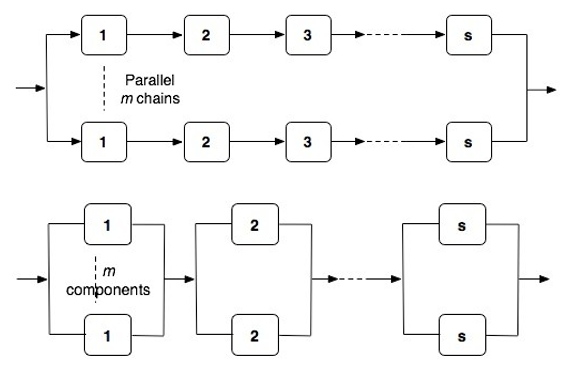
\includegraphics[width=0.7\textwidth]{img/hw5/es2.png}
	\caption{\textit{Reliability Block Diagrams Es.2}}
\end{figure}
\subsection{Svolgimento}
In entrambi i sistemi si possono riconoscere facilmente le parti che hanno componenti in serie e in parallelo. Non c'è bisogno di utilizzare tecniche come \textit{Legge di Bayes} o \textit{Teorema dell'Upperbound} per ricavare la legge della reliability complessiva.
\subsubsection{Sistema A}
Per "Sistema A" si intende il sistema in alto che compare in Fig.\ref{es2}.
\\Per $m=3$ e $s=4$ esso ha 4 componenti in serie, disposti all'interno di 3 blocchi in parallelo. Quindi:
\begin{equation*}
	\begin{split}
			&R_{serie} = \prod_{i=1}^{4} R_i = R^4 \\
			&R_{parallelo} = 1 - \prod_{j=1}^{3}(1-R_{serie}) = (1-R_{serie})^3 \\
			&R_A = 1-(1-R^4)^3
	\end{split}
\end{equation*}
\subsubsection{Sistema B}
Per "Sistema B" si intende il sistema in basso che compare in Fig.\ref{es2}.
\\Per $m=3$ e $s=4$ esso ha 4 blocchi in serie, ognuno dei quali contine 3 componenti in parallelo. Quindi:
\begin{equation*}
	\begin{split}
		&R_{parallelo} = 1 - \prod_{j=1}^{3}(1-R_{j}) = 1-(1-R)^3 \\
		&R_{serie} = \prod_{i=1}^{4}R_{parallelo} = R_{parallelo}^4 \\
		&R_B = [1-(1-R)^3]^4
	\end{split}
\end{equation*}
\vspace{0.5cm}
\\Dato che le due reliability $R_A$ e $R_B$ sono in funzione del \textit{mission time} $t$, per confrontarle si può valutare un grafico per vari valori del tempo $t$.
Sapendo che:
\begin{equation*}
	MTTF = 100h \quad \Rightarrow \quad \lambda = \dfrac{1}{100h}
\end{equation*}
Si ha:
\begin{equation}
	\begin{split}
			&R_A(t) = 1 - (1 - e^{-4\lambda t})^3 \\
			&R_B(t) = [1-(1-e^{-\lambda t})^3]^4
	\end{split}
\end{equation}
Con un semplice script MATLAB:
\begin{minted}[framesep = 1mm,
	fontsize = \footnotesize,
	breaklines,
	]{MATLAB}
MTTF = 100; % [h]
lambda = 1/MTTF;
m = 3; s = 4;
t = 0:1:200;
R = exp(-lambda*t);  %PDF

R1 = 1-(1-R.^s).^(m);   % Reilability del Sistema 1
R2 = (1-(1-R).^m).^s;   % Reilability del Sistema 2

figure;
plot(t,R1); hold on; plot(t,R2);
legend("Sistema Serie (A)", "Sistema Parallelo (B)");
grid;
\end{minted}
Fornendo come risultato il seguente grafico.
\begin{figure}[H]
	\centering
	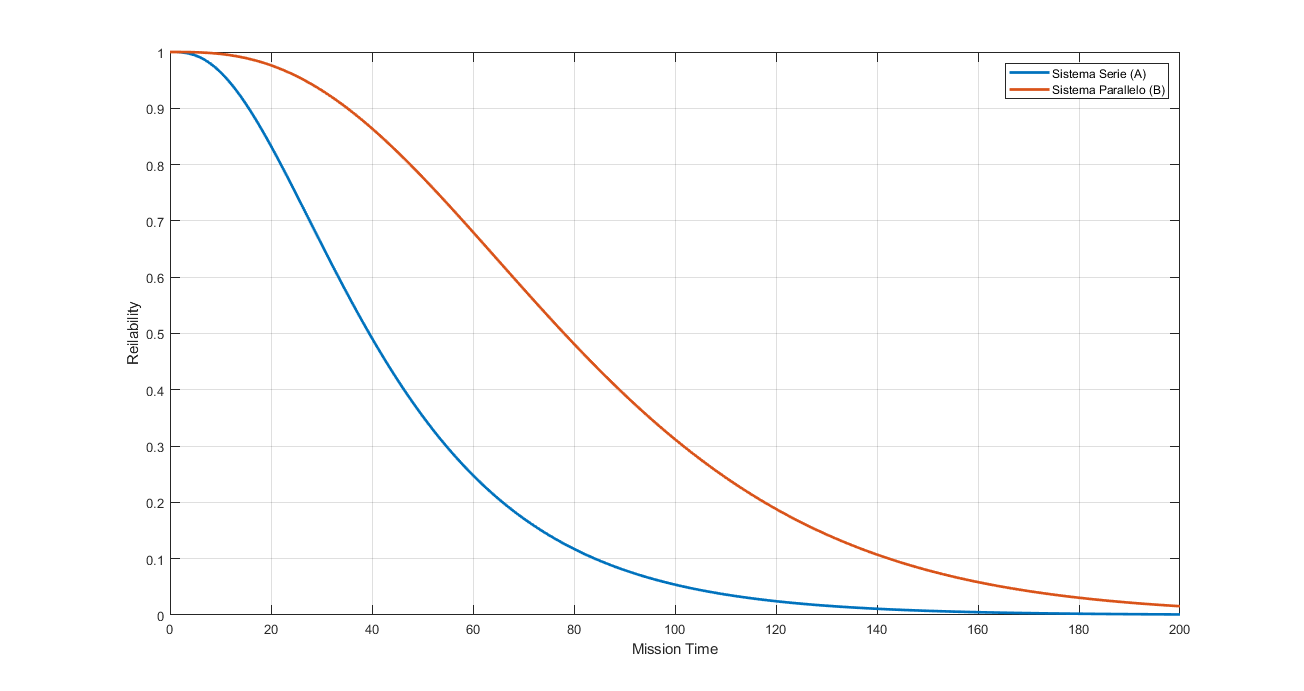
\includegraphics[width=\textwidth]{img/hw5/es2_grafico1.png}
	\caption{\textit{Confronto tra le reliability}}
\end{figure}
Come si può notare il "Sistema B" ha una reliability sempre maggiore rispetto al "Sistema A", per ogni \textit{mission time}. In realtà la stessa considerazione poteva essere fatta anche senza calcolare le due espressioni $R_A$ e $R_B$, poiché il secondo sistema ha un numero di \textit{success path} pari a $m^s$ mentre il primo sistema pari a $m$. Di conseguenza essendoci più percorsi alternativi, l'affidabilità è sicuramente maggiore.

\vspace{0.5cm}
Il "Sistema A" può essere opportunamente modificato per raggiungere la stessa reliability del "Sistema B" a parità di \textit{mission time}. Dato che il parametro $s$ non può essere cambiato (vincolo definito dalla traccia) l'unico parametro che può variare è $m$, ovvero il numero di blocchi in parallelo. 
\\$R_A$ e $R_B$ non sono la stessa funzione, quindi non esiste nessun valore di $m$ per cui le due funzioni si sovrappongono. Per raggiungere la stessa reliability allora bisogna prima fissare il \textit{mission time} e poi calcolare l'$m$ necessario. \\Per far ciò, in linea generale, posto $k$ come il numero di blocchi-serie da mettere in parallelo deve accadere:
\begin{equation}
	\begin{split}
		&1-(1-R(t)^s)^k = R_B(t) \\
		&1-R_B(t) = (1-R(t)^s)^k \\
		&k = \dfrac{ln(1-R_B(t))}{ln(1-R(t)^s)} 
	\end{split}
\end{equation}
Quindi $k$ dipende dal \textit{mission time}. Effettuando un grafico del valore di $k$ per vari istanti di tempo $t$, nel caso in esame con $m=3$ e $s=4$:
\begin{figure}[H]
	\centering
	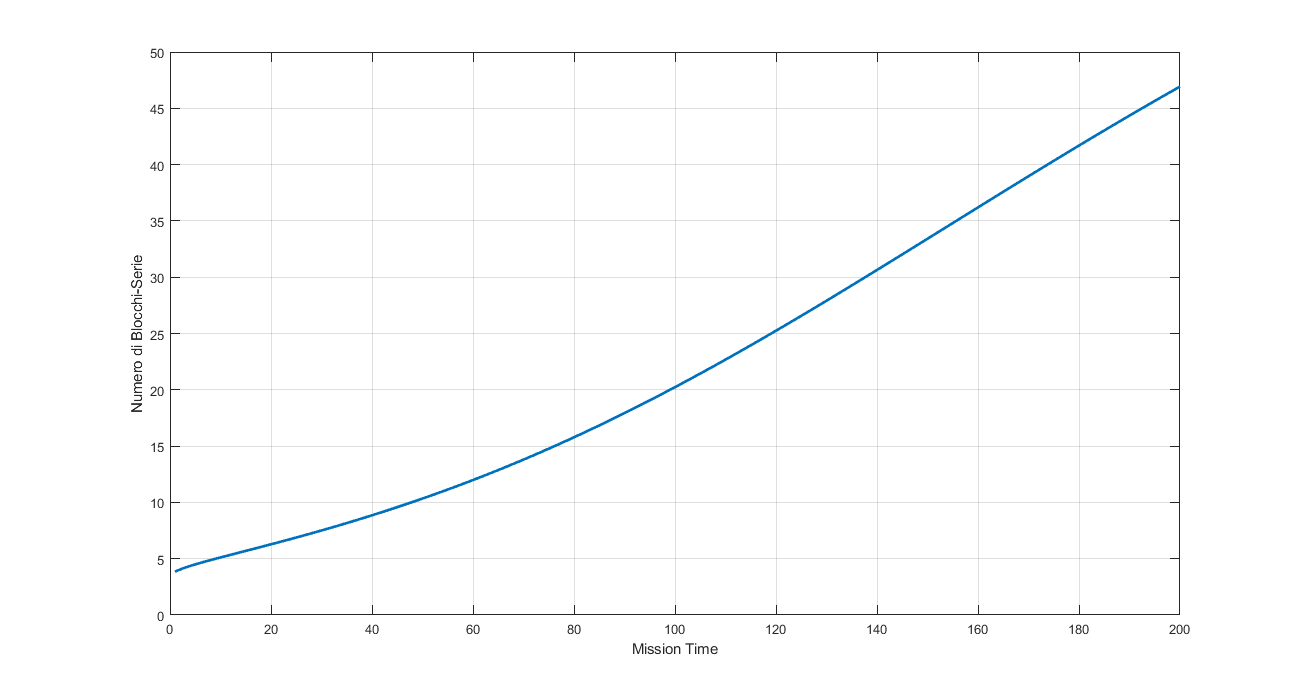
\includegraphics[width=\textwidth]{img/hw5/es2_grafico2.png}
	\caption{\textit{Numero di Blocchi-Serie in funzione del Mission Time}}
\end{figure}
Se si volesse avere quindi la stessa reliability per i due sistema con $t=100$ (ore) allora $k\approx20$, servendosi di circa $20\times 4 = 80$ componenti.
\begin{figure}[H]
	\centering
	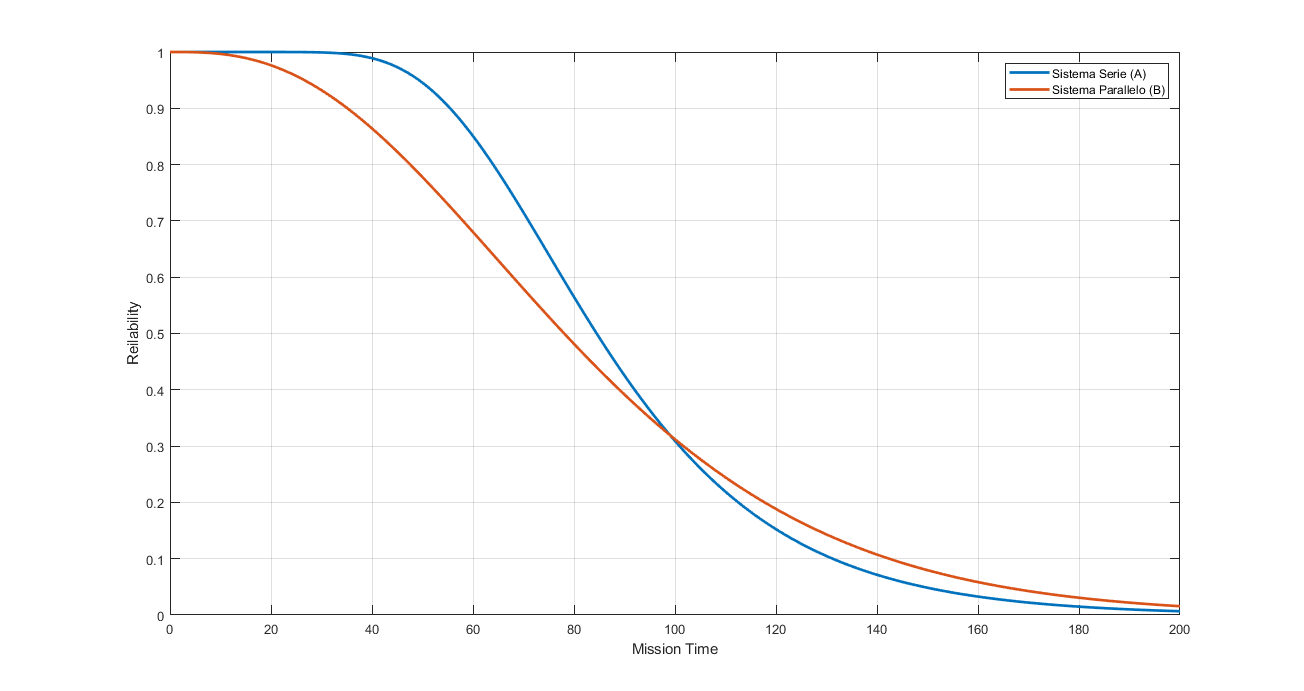
\includegraphics[width=\textwidth]{img/hw5/es2_grafico3.png}
	\caption{\textit{Confronto tra le reilability dei due sistemi}}
\end{figure}

\section{Esercizio 3}
L'architettura di una rete di computer in un sistema bancario e la seguente. L'architettura è chiamata \textbf{Skip-Ring Network} ed è progettata per consentire ai componenti di comunicare anche in presenza di nodi falliti.
\\Per esempio, se il \textit{Nodo 1} fallisce, il \textit{Nodo 8} può oltrepassare il nodo fallito attraverso un link alternativo, potendo raggiungere il \textit{Nodo 2}. 
\\Assumendo che tutti i link sono perfetti e ogni nodo ha una reilability $R_m$, ricavare l'espressione della reilability della rete.
\\Se $R_m$ ha una legge di fallimento esponenziale e il \textit{failure rate} di ogni nodo è di 0.005 fallimenti per ora, determinare la reilability del sistema dopo un periodo di 48 ore.
\begin{figure}[H]
	\centering
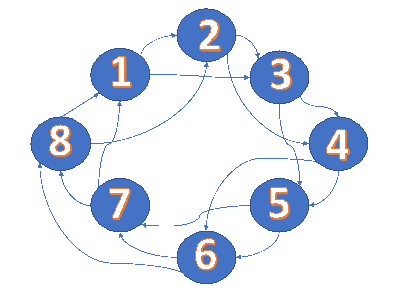
\includegraphics[width=0.7\textwidth]{img/hw5/es3_traccia.png}
\caption{\textit{Traccia}}
\end{figure}

\subsubsection{Svolgimento}
Il sistema funziona anche in presenza di nodi guasti, purché non si guastino nodi consecutivi. In tale scenario infatti l'anello viene interrotto e il sistema smette di funzionare. Sulla base di questo si può notare che il sistema continua a funzionare anche se falliscono 4 nodi, purché non siano consecutivi.
\\Per ricavare la legge della reilability ci si può ispirare alla legge per un sistema generale \textit{M-out-of-N} in cui $M$ sono il numero di nodi che devono funzionare, su $N$ affinché il sistema continua a funzionare.
\\In questo caso $M=4$ e $N=8$, a causa del fatto che se falliscono più di 4 nodi, automaticamente almeno due nodi falliti saranno consecutivi, interrompendo l'anello.
\begin{equation*}
	R_{sys} = \sum_{i=0}^{N-M}g(i)R_m^{N-i}(1-R_m)^i
\end{equation*}
in cui $i$ indica il numero di nodi falliti e $g(i)$ indica il numero di permutazioni di quel fallimento.
\\Nel caso specifico:
\begin{equation*}
	R_{sys} = \sum_{i=0}^{4}g(i)R_m^{N-i}(1-R_m)^i
\end{equation*}
\begin{itemize}
	\item i=0. Nessun nodo è guasto.
	\begin{equation*}
		g(0) = 1 
	\end{equation*}
	Poiché è un evento che non dipende dal numero dei nodi. La reilability al'iterazione 0 vale:
	\begin{equation*}
		R_{sys}[0] = R_m^8
	\end{equation*}
	\item i=1. Un solo nodo è guasto. Il sistema continua a funzionare normalmente. Al massimo si possono guastare $N$ nodi.
	\begin{equation*}
		g(1) = 8
	\end{equation*}
	La reilability vale:
	\begin{equation*}
	R_{sys}[1] = 8 R_m^7 (1-R_m)
	\end{equation*}	
	\item i=2. Due nodi sono guasti. In questo caso bisogna prestare attenzione. Il sistema continua a funzionare se i nodi guasti non sono adiacenti. Il numero di permutazioni vale come tutte le possibili permutazioni dei due nodi, sottratto il numero di combinazioni in cui i due nodi sono adiacenti:
	\begin{equation*}
		g(2) = \begin{pmatrix}
			8 \\ 2
		\end{pmatrix} - 8 = 20
	\end{equation*}
	Quindi:
	\begin{equation*}
		R_{sys}[2] = 20 R_m^6 (1-R_m)^2
	\end{equation*}	
	\item i=3. Se falliscono 3 nodi, come prima, bisogna stare attenti a considerare solo le combinazioni per cui non ci siano due nodi guasti consecutivi. Al totale delle combinazioni devono essere sottratte:
	\begin{enumerate}
		\item Combinazioni in cui 3 nodi sono adiacenti, come nel caso precedente, ovvero 8 combinazioni.
		\item Combinazioni in cui 2 nodi sono adiacenti e il terzo non è adiacente. Fissati due nodi adiacenti, il terzo non è adiacente solo in 4 casi. \\Ad esempio se il \textit{Nodo 2} e il \textit{Nodo 3} sono guasti, il terzo nodo deve essere tra \textit{Nodo 5}, \textit{Nodo 6}, \textit{Nodo 7}, \textit{Nodo 8}. Dato che può capitare per 8 volte, allora si hanno $8*4=32$ combinazioni.
	\end{enumerate}
	\begin{equation*}
		g(3) = \begin{pmatrix}
			8 \\ 3
		\end{pmatrix} - 8 - 32 = 16
	\end{equation*}
	\begin{equation*}
		R_{sys}[3] = 16 R_m^5 (1-R_m)^3
	\end{equation*}	
	\item i=4. Quattro nodi guasti. Questo è un caso limite, poiché i quattro nodi guasti devono alternarsi tra loro, altrimenti si avranno necessariamente due nodi guasti adiacenti. Quindi esistono solo due combinazioni:
	\begin{enumerate}
		\item Nodi: 1-3-5-7
		\item Nodi: 2-4-6-8
	\end{enumerate}
	\begin{equation*}
	g(4) = 2
	\end{equation*}
	Per cui:
	\begin{equation*}
		R_{sys}[4] = 2 R_m^4 (1-R_m)^4
	\end{equation*}
\end{itemize}
Avendo calcolato il vettore $g(i)$ la reilability complessiva vale:
\begin{equation*}
	R_{sys} = R_m^8 + 8 R_m^7 (1-R_m) + 20 R_m^6 (1-R_m)^2 + 16 R_m^5 (1-R_m)^3 + 2 R_m^4 (1-R_m)^4
\end{equation*}
Dato che si conosce il failure rate, e ogni componente ha una legge di reilability esponenziale:
\begin{equation*}
	R_m = e^{-\lambda t} = e^{-0.005 t}
\end{equation*}
Per cui il grafico complessivo di $R_{sys}$ è il seguente.
\begin{figure}[H]
	\centering
	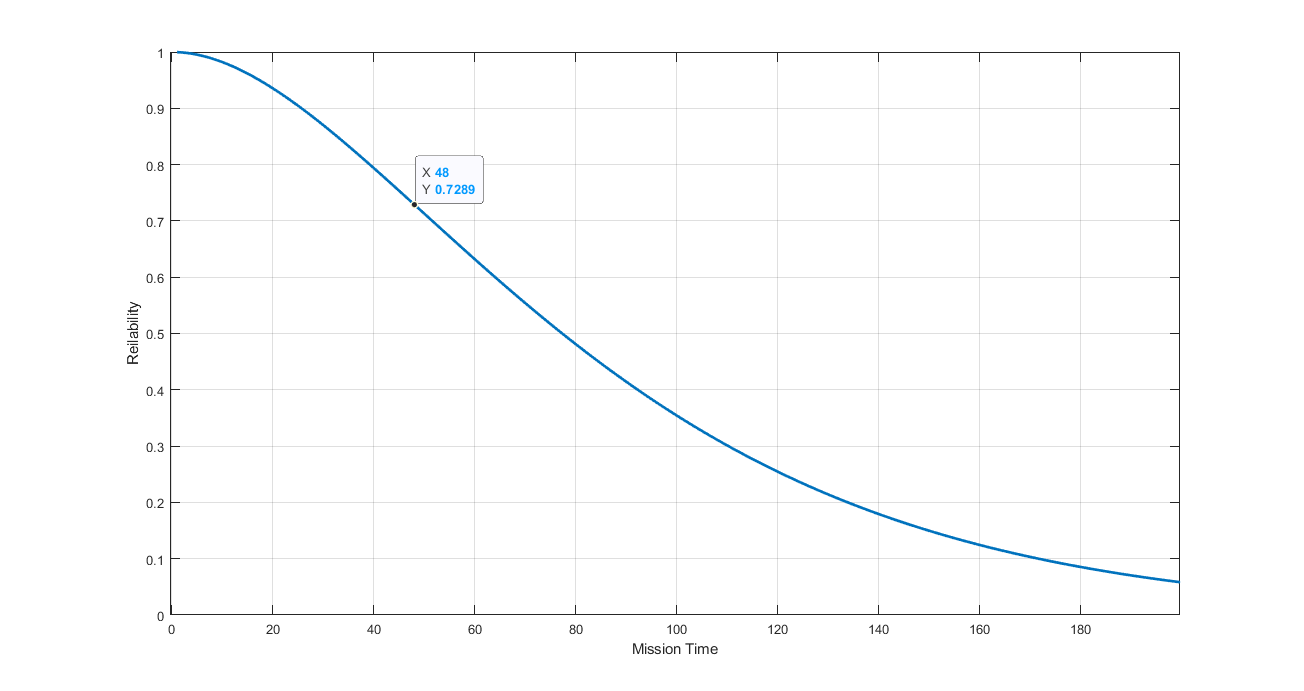
\includegraphics[width=\textwidth]{img/hw5/es3_grafico.png}
	\caption{\textit{Reilabilty del sistema}}
\end{figure}
Inoltre dopo 48h di lavoro, il sistema ha una reilability pari a:
\begin{equation*}
	R_sys(48) \approx 0,7289
\end{equation*}

\section{Esercizio 4}
Confrontare la reilability dei seguenti sistemi, assumendo un \textit{Mean Time to Failure} esponenziale, con i seguenti valori:
\begin{itemize}
	\item \textit{$MTTF_A$ = 1000h}
	\item \textit{$MTTF_B$ = 9000h}
	\item \textit{$MTTF_C$ = 2000h}
\end{itemize}
\begin{figure}[H]
	\centering
	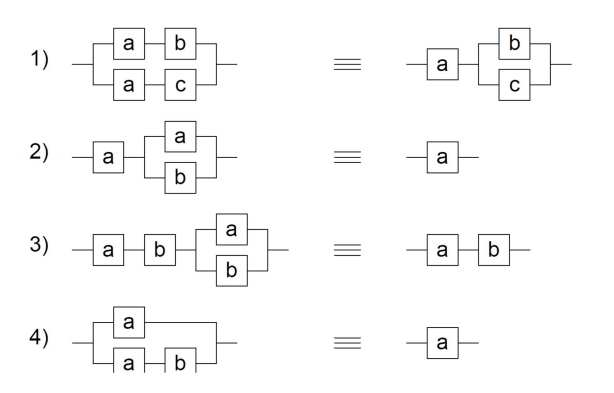
\includegraphics[width=0.8\textwidth]{img/hw5/es4_traccia.png}
	\caption{\textit{Sistemi da confrontare}}
\end{figure}
\subsection{Svolgimento}
Innanzitutto sono state calcolati tassi di fallimento $\lambda$:
\begin{equation*}
	\begin{split}
		&\lambda_A = \frac{1}{MTTF_A} = \frac{1}{1000h}\\
		&\lambda_B = \frac{1}{MTTF_B} = \frac{1}{9000h}\\
		&\lambda_C = \frac{1}{MTTF_C} = \frac{1}{2000h}
	\end{split}
\end{equation*}
e di conseguenza le reliability relative ad ogni singolo componente:
\begin{equation*}
	\begin{split}
		&R_A(t) = e^{-\lambda_A t} = e^{-\frac{1}{1000h} t}\\
		&R_B(t) = e^{-\lambda_B t} = e^{-\frac{1}{9000h} t}\\
		&R_C(t) = e^{-\lambda_C t} = e^{-\frac{1}{2000h} t}
	\end{split}
\end{equation*}
\subsubsection{Confronto 1}
Confrontiamo il parallelo tra le serie (A e B) e (A e C), con la serie tra il blocco A e il parallelo tra i blocco B e C.
Reliability \textbf{sistema 1}:
\begin{equation*}
	\begin{split}
		&R11(t) = 1-(1-R_A*R_B)*(1-R_A*R_C) = \\
		&1-(1-e^{-\frac{1}{1000h} t}*e^{-\frac{1}{9000h} t})*(1-e^{-\frac{1}{1000h} t}*e^{-\frac{1}{2000h} t}) = 1 -(1-e^{\frac{1}{900h} t})(1-e^{-\frac{3}{2000h}t}) = \\
		&e^{-\frac{3}{2000h}t}+e^{-\frac{1}{900h}t}-e^{-\frac{47}{18000h}t}
	\end{split}
\end{equation*}
Reilability \textbf{sistema 2}:
\begin{equation*}
	\begin{split}
		&R12(t) = R_A * [1-(1-R_B)*(1-R_C)] = e^{-\frac{1}{1000h} t}*[1-(1-e^{-\frac{1}{9000h} t})*(1-e^{-\frac{1}{2000h} t})] = \\
		& e^{-\frac{3}{2000h}t}+e^{-\frac{1}{900h}t}-e^{-\frac{29}{18000h}t}
	\end{split}
\end{equation*}
\begin{figure}[H]
	\centering
	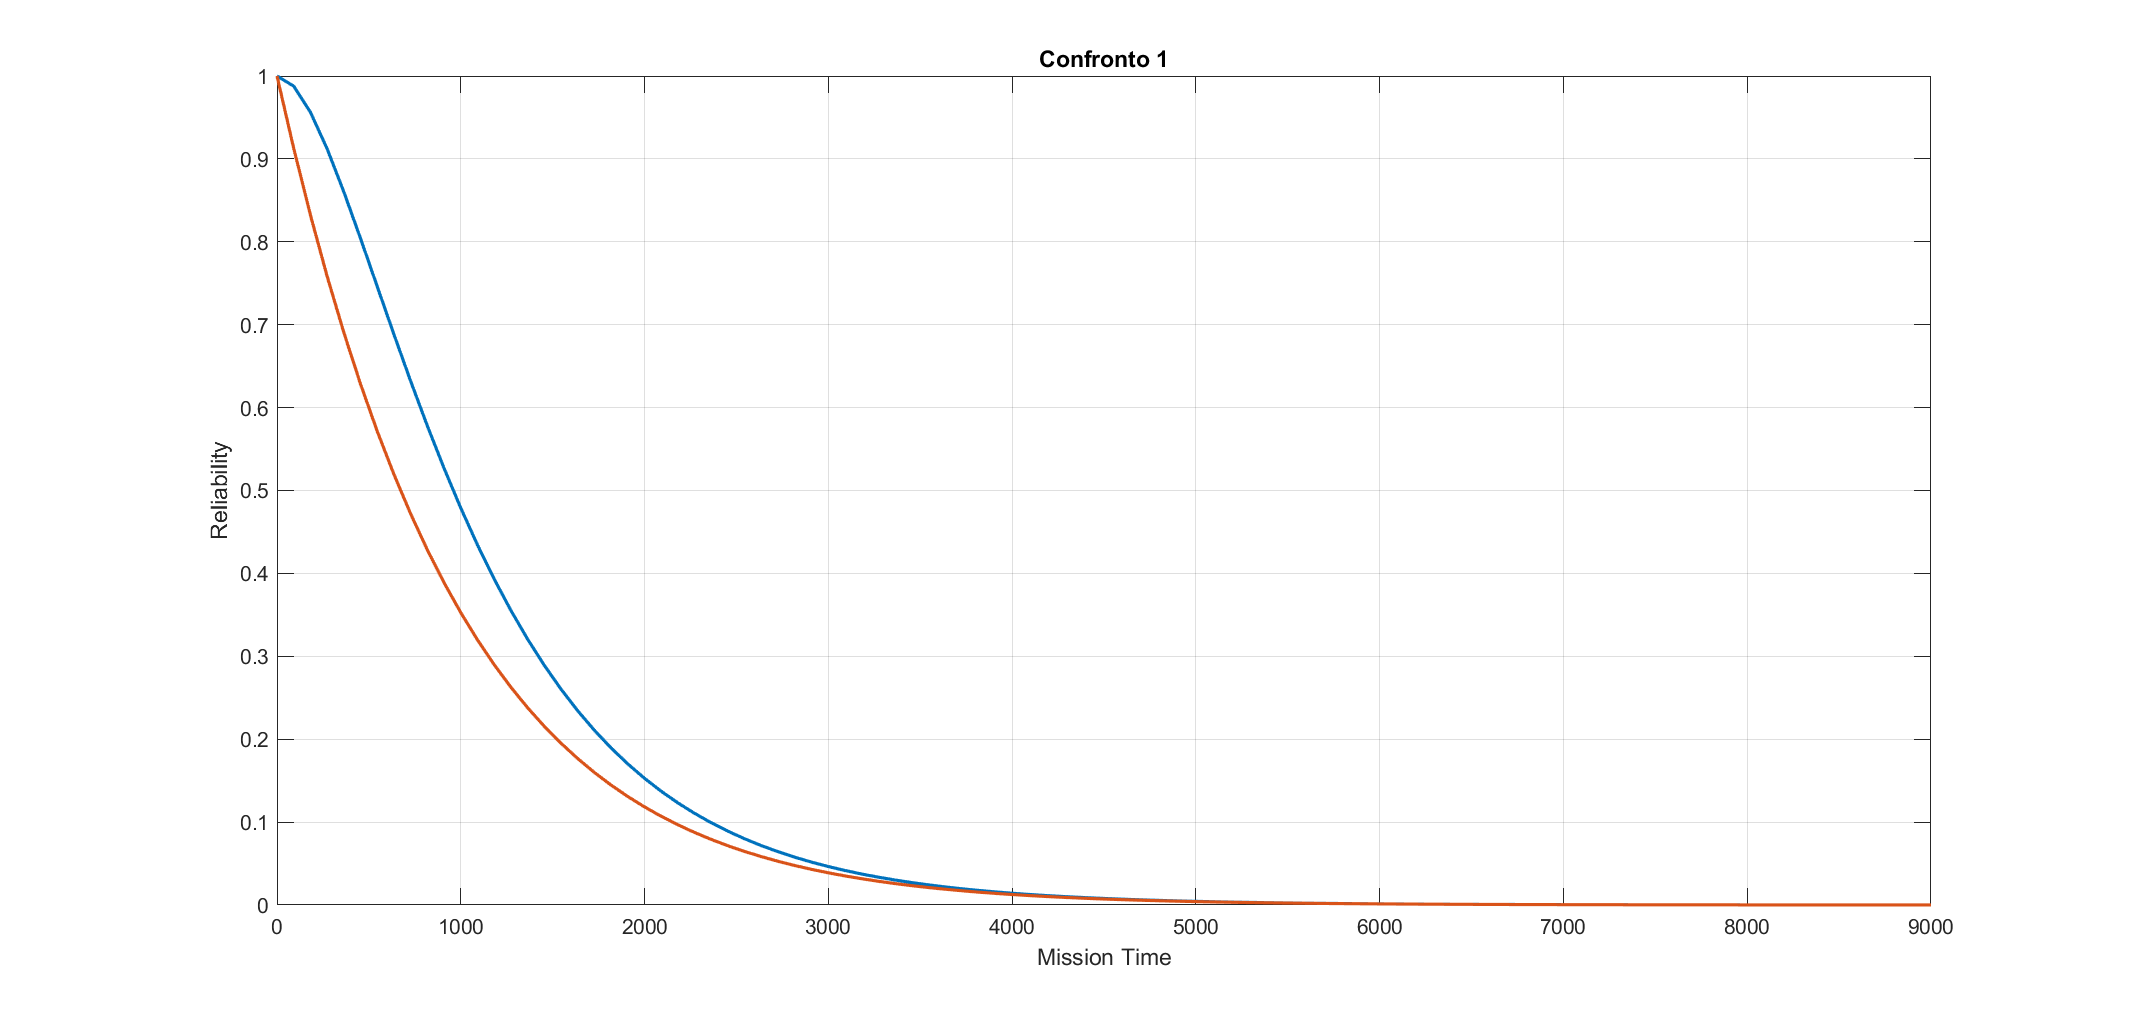
\includegraphics[width=\textwidth]{img/hw5/es4_1.png}
	\caption{\textit{Primo confronto}}
\end{figure}
La reliability del primo sistema (in blu nel grafico) risulta, con evidenza, maggiore rispetto a quella del secondo, fino a valori di t pari a circa 4000h.
\subsubsection{Confronto 2}
Nel secondo punto confrontiamo la reliability del blocco A messo in serie ad un parallelo tra A e B, con quella del singolo blocco A. 
\\
Reliability \textbf{sistema 1}:
\begin{equation*}
	\begin{split}
		&R21= R_A*[1-(1-R_A)*(1-R_B)] =e^{-\frac{1}{1000h} t}*[1-(1-e^{-\frac{1}{1000h} t})*(1-e^{-\frac{1}{9000h} t})] = \\
		&e^{-\frac{1}{900h}t}+e^{-\frac{1}{500h}t}+e^{-\frac{19}{9000h}t}
	\end{split}
\end{equation*}
Reliability \textbf{sistema 2}:
\begin{equation*}
	R22 = R_A = e^{-\frac{1}{1000h}}
\end{equation*}
\begin{figure}[H]
	\centering
	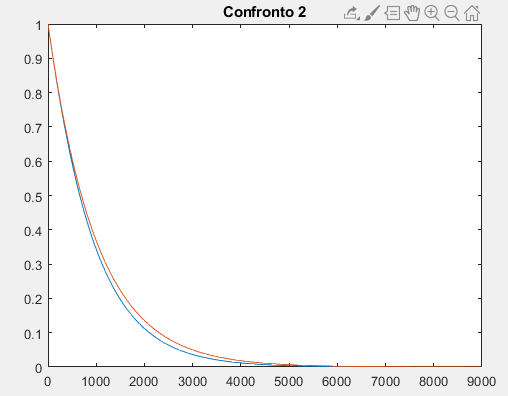
\includegraphics[width=\textwidth]{img/hw5/es4_2.png}
	\caption{\textit{Secondo confronto}}
\end{figure}
La reliability del blocco A, per valori di mission time compresi tra 1000h e 5000h circa, risulta essere maggiore di quella del sistema 1.
\subsubsection{Confronto 3}
In questo caso viene confrontato un primo sistema composto dai blocchi A e B in serie tra di loro e a sua volta in serie con il loro parallelo, ed un secondo sistema formato dalla semplice serie tra A e B.
\\
Reliability \textbf{sistema 1}:
\begin{equation*}
	\begin{split}
		&R31 = R21*R_B = e^{-\frac{1}{1000h} t}*e^{-\frac{1}{9000h} t}*[1-(1-e^{-\frac{1}{1000h} t})*(1-e^{-\frac{1}{9000h} t})] = \\
		&e^{-\frac{11}{9000h}t}+e^{-\frac{19}{9000h}t}+e^{-\frac{2}{900h}t}
	\end{split}
\end{equation*}
Reliability \textbf{sistema 2}:
\begin{equation*}
	\begin{split}
		&R32 = R_A*R_B = e^{-\frac{1}{1000h} t}*e^{-\frac{1}{9000h} t} = e^{-\frac{1}{900h}t}
	\end{split}
\end{equation*}
\begin{figure}[H]
	\centering
	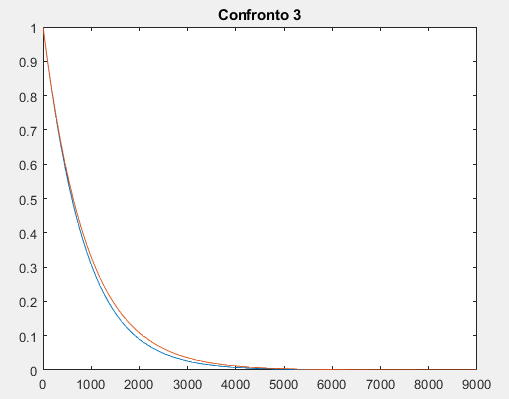
\includegraphics[width=\textwidth]{img/hw5/es4_3.png}
	\caption{\textit{Terzo confronto}}
\end{figure}
Nel primo sistema (in blu), la serie con il parallelo implica una riduzione della reilability per mission time compresi tra 1000h e 5000h circa.
\subsubsection{Confronto 4}
Infine viene confrontato il parallelo tra il blocco A e la serie tra A e B, con il singolo blocco A.
\\
Reliability \textbf{sistema 1}:
\begin{equation*}
	\begin{split}
		&R41 = 1-(1-R_A)*(1-R_A*R_B) = 1-(1-e^{-\frac{1}{1000h} t})*(1-e^{-\frac{1}{1000h} t}*e^{-\frac{1}{9000h} t}) = \\
		&e^{-\frac{1}{900h}t}+e^{-\frac{1}{1000h}t}-e^{-\frac{19}{9000h}t}
	\end{split}
\end{equation*}
Reliability \textbf{sistema 2}:
\begin{equation*}
	R42 = R_A = e^{-\frac{1}{1000h}}
\end{equation*}
\begin{figure}[H]
	\centering
	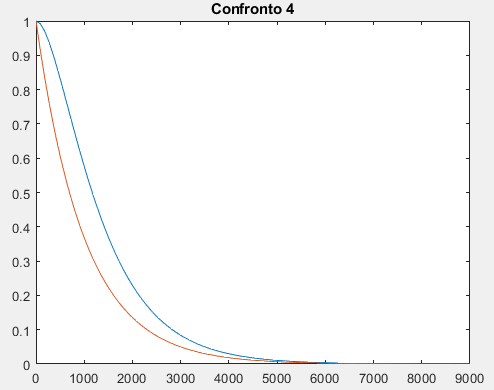
\includegraphics[width=\textwidth]{img/hw5/es4_4.png}
	\caption{\textit{Quarto confronto}}
\end{figure}
La reliability del primo sistema risulta incrementata rispetto a quella del blocco A, come conseguenza del parallelo tra i blocchi.
\section{Esercizio 5}
Il sistema mostrato nella figura sottostante è un sistema di elaborazione per un elicottero. Esso ha due processori e due terminali ridondanti. Sono utilizzati due bus, anch'essi dual-redundant. La parte interessante del sistema è il "navigation equipment". Il velivolo può essere completamente navigato utilizzando l' \textit{Inertial Navigation System (INS)}. Se l'INS fallisce, il velivolo può essere navigato utilizzando la combinazione del \textit{Doppler} con l' \textit{Altitude Heading and Reference System (AHRS)}. Il sistema contiene 3 unità AHRS, delle quali solo una è necessaria. Questo è un esempio di ridondanza funzionale dove i dati provenienti dall'AHRS e dal Doppler possono essere utilizzati per rimpiazzare l'INS, se esso fallisce. A causa di altri sensori e strumenti, entrambi i bus sono necessari per il funzionamento del sistema a prescindere dalla modalità di navigazione.
\begin{figure}[H]
	\centering
	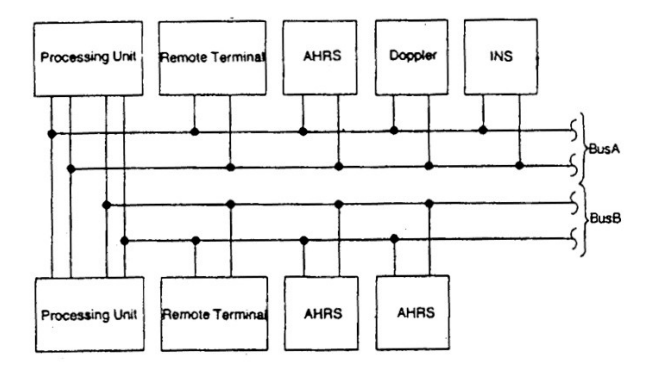
\includegraphics[width=0.7\textwidth]{img/hw5/es5_traccia.png}
	\caption{\textit{Processing system for a helicopter}}
\end{figure}
\subsection{Punto A: Disegnare il Reilability Block Diagram del Sistema}
Possiamo suddividere il sistema in cinque "macro-blocchi":
\begin{enumerate}
	\item \textbf{Bus A}.
	\item \textbf{Bus B}.
	\item \textbf{Sistema di navigazione}.
	\item \textbf{Processing unit}.
	\item \textbf{Remote terminal}.
\end{enumerate}
Se almeno uno di essi fallisce, il sistema intero fallisce. Ogni macro-blocco, (eccetto il sistema di navigazione per il quale è stata pensata una particolare ridondanza funzionale descritta nella traccia), è dual-redundant. Inoltre, ciascuna delle due \textit{Processing Unit} è connessa ad entrambi i bus, in modo da avere dual-redoundance sul singolo bus. 
\\
\\
Partendo da queste informazioni è stato realizzato il \textit{Reliability Block Diagram}:
\\immagine diagramma
\subsection{Punto B: Disegnare il Fault Tree del Sistema e analizzare i minimal cutsets}
Partendo dal Reliability Block Diagram è possibile ricavare il rispettivo Fault Tree, considerando che il sistema fallisce se il \textit{Top Level Event} ha valore logico 1.
\\In particolare lo serie saranno sostituite con delle porte OR, mentre i paralleli con porte END. 
\\immagine fault tree
\\espressione logica del fault tree 
\\discussione sui minimal cutsets = combinazione di eventi base che portano al fallimento (mi esce un 1 nel TLE)
\subsection{Punto C}
\subsection{Punto D}
